\chapter{Introduction to LBNF and DUNE}
\label{ch:project-overview}

%%%%%%%%%%%%%%%%%%%%%%%%%%%%%%%%%%%%%%%%%%%%%%%%%%%%%%%%%%%%%%%
\section{International Convergence}

During the last decade, several independent worldwide efforts have attempted to develop paths towards a next-generation long-baseline neutrino experiment, including in the U.S. with LBNE, in Europe with LBNO and in Japan with Hyper-Kamiokande. The community has generally recognized that putting in place  
the conditions necessary to 
execute this challenging science program in a comprehensive way requires previously independent 

efforts to converge. 

In this context, the Deep Underground Neutrino Experiment (DUNE) represents the convergence of a substantial fraction of the worldwide neutrino-physics community around the 
opportunity provided by the 
large investment planned by the U.S. Department of Energy (DOE) to support 
a significant expansion of the underground infrastructure at the Sanford Underground Research 
Facility (SURF) in South Dakota, \SI{1300}{\km} from Fermilab, and to create a megawatt neutrino-beam facility at Fermilab by 2026.  The PIP-II accelerator upgrade~\cite{pip2-2013} at 
Fermilab will drive the new neutrino beamline at Fermilab with a beam power\footnote{assuming a \SI{120}{\GeV} primary proton beam. For a \SI{80}{\GeV} primary proton beam, the corresponding beam power is \SI{1.07}{\MW}.} of up to \SI{1.2}{\MW}, with a planned upgrade 
of the accelerator complex to enable it to provide up to \SI{2.4}{\MW} of beam power by 2030.  

This document presents 
the Conceptual Design Report (CDR) put forward by an international neutrino community to pursue 
the Deep Underground Neutrino Experiment at the Long-Baseline Neutrino Facility (LBNF/DUNE),
a groundbreaking science experiment for long-baseline neutrino oscillation studies and for neutrino astrophysics and nucleon decay searches. The DUNE far detector will be a very large modular liquid argon time-projection chamber (LArTPC) located deep underground, coupled to the LBNF multi-megawatt   
wide-band neutrino beam.   DUNE will also have a high-resolution and high-precision near detector.

The physics case for the LBNF neutrino facility was highlighted as a strategic priority in the 2014 P5 report~\cite{p5report2014}.
P5 identified the following minimum requirements for LBNF to proceed: 
the identified capability to reach an exposure of at least 120~\ktMWyr{}~\footnote{An exposure
of 1 MW.year corresponds to $1\times 10^{21}$ protons-on-target per year at 120 GeV. This includes the LBNF beamline efficiency which is estimated to be 56\%.}  by the 2035 timeframe;
the far detector situated underground with cavern space for expansion to at least 40-kt LAr fiducial;
1.2-MW beam power upgradable to multi-megawatt power;
demonstrated capability to search for supernova bursts; and
a demonstrated capability to search for proton decay, 
providing a significant improvement in discovery sensitivity over current searches for the proton lifetime.
Furthermore, P5 identified  the \textit{goal} of a sensitivity to CP violation of better than 3$\sigma$ over more than 75\% 
of the range of possible values of the unknown CP-violating phase \deltacp.
The strategy presented in this CDR meets all of these requirements.


%%%%%%%%%%%%%%%%%%%%%%%%%%%%%%%
\section{About this Document}

This document, an update to \volintro,~\cite{lbnecdr} provides an overview of LBNF and
DUNE (Chapter~\ref{ch:project-overview}), including the strategy that is being developed to construct, install and commission the technical and conventional facilities in accordance with the requirements set out by the P5 report of 2014~\cite{p5report2014}, which, in turn, is in line with the CERN
European Strategy for Particle Physics (ESPP) of 2013~\cite{ESPP-2012}. This volume also introduces the DUNE science program (Chapter~\ref{v1ch:science}) and the technical designs of the facilities and the detectors 
(Chapter~\ref{v1ch:tech-designs}). It concludes with a description of the LBNF and DUNE organization and management structures (Chapter~\ref{v1ch:org-mgmt}).



%%%%%%%%%%%%%%%%%%%%%%%%%%%%%%%%%%%%%%%%%%%%%%%%%%%%%%%%%%%%%%%%
\section{A Compelling Scientific Program}

The study of the properties of neutrinos has produced 
many surprises, including the evidence for physics beyond the Standard Model of elementary particles and interactions.   The phenomenon of neutrino flavor oscillations, whereby 
neutrinos can transform into a different flavor after traveling a distance, 
is now well established. Important conclusions that follow from these discoveries include that neutrinos have mass and that their 
mass eigenstates are mixtures of their  
flavor eigenstates.

Speculations on the origin of neutrino masses and mixings are wide-ranging. 
Solving the puzzle will require more precise and detailed experimental information with neutrinos and antineutrinos and with sensitivity to matter effects. With the exception of a few anomalous results, the current data can be described in terms of the three-neutrino paradigm, in which the 
quantum-mechanical mixing of the three mass eigenstates produces the three known neutrino-flavor states.  The mixings are described by the Pontecorvo-Maki-Nakagawa-Sakata (PMNS) matrix, a parameterization that includes a CP-violating phase. 

The primary science objectives  
of DUNE are to carry out a comprehensive investigation of neutrino oscillations to test CP violation in the lepton sector, determine the ordering of the neutrino masses, and to test the three-neutrino paradigm.
By measuring \textit{independently} the  propagation of neutrinos and antineutrinos through matter, DUNE will be able to observe neutrino transitions with the precision required to determine the 
CP-violating phase and  
the neutrino mass hierarchy.

The construction of LBNF and DUNE will also enable a high-priority ancillary science program, such as 
very precise measurements of neutrino interactions and cross-sections, studies of nuclear effects in such interactions, measurements of the structure of nucleons, as well as precise tests of the electroweak theory. 
These measurements of the properties of neutrino interactions are also necessary 
to achieve the best sensitivities in the long-baseline neutrino oscillation program. 

The DUNE far detector, consisting of four LArTPC modules located deep underground, each with a mass forty times larger than ever before built,  
will offer unique capabilities for addressing 
non-accelerator physics topics. These include measuring atmospheric neutrinos, searching for nucleon decay, and measuring astrophysical neutrinos --- possibly even the neutrino burst from a core-collapse supernova. 
Observations of these kinds will bring new insight into these fascinating natural phenomena. 


An intriguing conjecture is that of neutrino masses being related to an 
ultra-high-energy scale that may be associated with the unification of matter and forces. Such theories are able to describe the absence of antimatter in the universe in terms of the properties of ultra-heavy particles; they also  
offer an explanation  
of cosmological inflation in terms of the phase transitions associated with the breaking of symmetries at this ultra-high-energy scale. DUNE's capability to detect and study rare events such as nucleon decays in an unbiased and unprecedented way will allow it to probe these very high-energy scales. 


Finally, further developments of LArTPC  
technology during the course of the DUNE far detector construction may open up the opportunity
to observe very low-energy phenomena such as solar neutrinos or even the diffuse supernova neutrino flux.


%%%%%%%%%%%%%%%%%%%%%%%%%%%%%%%%%%%%%%%%%%%%%%%%%%%%%%%%%%%%%%%
\section{Overall LBNF/DUNE Project Strategy} 

The LBNF/DUNE Project (the ``Project'') strategy presented in this CDR has been developed to meet the requirements 
set out in the P5 report and 
takes into account the recommendations of the CERN European Strategy for Particle 
Physics (ESPP) of 2013, which classified the long-baseline neutrino program as 
one of the four scientific objectives with required international infrastructure.

The Report of the Particle Physics Project Prioritization Panel (P5) 
states that for a long-baseline neutrino oscillation experiment, ``The 
minimum requirements to proceed are the identified capability to reach an exposure 
of \num{120}~\ktMWyr{} by the 2035 timeframe, the far detector situated underground 
with cavern space for expansion to at least 40~kt LAr fiducial volume, and 1.2~MW 
beam power upgradable to multi-megawatt power. The experiment should have the demonstrated 
capability to search for supernova bursts and for proton decay, providing a significant 
improvement in discovery sensitivity over current searches for the proton lifetime.'' 
Based on the resource-loaded schedules for the reference designs of the facility 
and the detectors~\cite{lbnf-cf-pdr, cryo-design-rpt, design-doc-dune-det}, 
the strategy presented here meets these criteria. 

With the availability of space for expansion and improved access at SURF, 
the international DUNE Collaboration proposes to construct a deep-underground neutrino observatory based on four independent \ktadj{10} LArTPCs at this site.   
The goal is the deployment of two \ktadj{10} fiducial mass detectors in a relatively short timeframe, followed by future expansion to the full detector size as soon thereafter as possible. 

Several LArTPC designs are under development by different groups worldwide, involving both single- and dual-phase readout technology.
The DUNE Collaboration has the necessary scientific and technical expertise,  
and international participation  to design and implement this exciting discovery experiment. 

The Long-Baseline Neutrino Facility (LBNF) provides
\begin{itemize}

\item  the  technical and conventional facilities for a powerful \MWadj{1.2} neutrino beam utilizing the PIP-II upgrade of the Fermilab accelerator 
complex, to become operational by 2025 
at the latest, and to be upgradable to \SI{2.4}{\MW} with the proposed 
PIP-III upgrade

\item  the civil construction (conventional facilities or CF) for the near detector systems at Fermilab 

\item the excavation of four underground caverns at SURF, planned to be completed 
by 2021 under a single contract; each cavern to be capable of housing a cryostat for
a minimum \ktadj{10} fiducial mass LArTPC


\item surface, shaft, and underground infrastructure to support 
the outfitting of the caverns with four free-standing, steel-supported cryostats 
and the required cryogenics systems. The first cryostat will be available for filling, after installation of the detector components, by
2023, enabling a rapid deployment of the first two \ktadj{10} far detector modules. 
The intention is to install the third and fourth cryostats as rapidly as funding will 
allow.

\end{itemize}

The Deep Underground Neutrino Experiment (DUNE) provides
\begin{itemize}

\item four massive LArTPCs, each with a fiducial mass of at least \SI{10}{\kt}. The division of 
the far detector into four equal-mass detectors provides the Project flexibility 
in the installation and funding (DOE vs. non-DOE); this division also mitigates risks and allows for an early and graded science return.

\item the near detector systems, consisting of a high-resolution neutrino detector 
and the muon monitoring system that will enable %necessary to reach 
the precision %requirements 
needed to fully 
exploit the statistical power of the %very massive 
far detector coupled to the %powerful 
MW-class 
neutrino beam
\end{itemize}


Based on the reference design described below and in Volumes 2, 3 and 4 of this 
CDR, the resource-loaded schedule plans for the first two \ktadj{10} far detector modules to be
operational by 2025, with first beam shortly afterward. At that time, the cavern 
space for all four \ktadj{10} far detector modules will be available, allowing for 
an accelerated installation schedule if sufficient funding sources for
the experiment can be established on an accelerated timescale.  

\vspace{6pt}
The Project strategy described above meets the experiment's scientific objectives,
 reaching an exposure of 
\num{120}~\ktMWyr{} by 2032, and potentially earlier if additional resources are identified. 
The P5 recommendation of sensitivity to CP violation of 3$\sigma$ for 75\% of $\delta_\text{CP}$
values can be reached with an exposure of \num{850}~\ktMWyr{} with an optimized beam.

%%%%%%%%%%%%%%%%%%%%%%%%%%%%%%%%%%%%%%%%%%%%%%%%%%%%%%%%%%%%%%%
\section{The International Organization and Responsibilities}

The 
model used by CERN for managing the construction and exploitation of the LHC and its experiments was used as a starting point for the joint management of LBNF and the experimental program.  Fermilab, as the host laboratory, has the responsibility for the facilities and their operations 
and oversight of the experiment and its operations.  Mechanisms to ensure input from and coordination among all of the funding agencies supporting the Collaboration, modelled on the CERN Resource Review Board, have been adopted. 
A similar structure is employed to coordinate among funding agencies supporting the LBNF construction and operation.  

The LBNF/DUNE Project will be organized as two distinct entities. The LBNF portion is funded primarily
by the U.S. DOE acting on behalf of the hosting country.  CERN provides in-kind contributions to the LBNF infrastructure needed for the DUNE experiment. The DUNE portion is organized
as an international collaboration; it is adopting a model in which the DOE and international funding agencies share costs  
for the DUNE detectors.

The DUNE Collaboration is responsible for
\begin{itemize}
\item the definition of the scientific goals and corresponding scientific and technical requirements on the detector systems and neutrino beamline
\item the design, construction, commissioning and operation of the detectors
\item the scientific research program conducted with the DUNE detectors 

\end{itemize}

The high-intensity proton source at Fermilab that will drive the long-baseline neutrino beam utilizes the existing 
Main Injector with upgraded injectors (PIP-II).  PIP-II is also being planned with significant international collaboration.  Fermilab, working with the participation and support of international partners, is responsible for 
LBNF, including
\begin{itemize}
\item design, construction and operation of the LBNF beamline, including the primary proton beamline and the neutrino beamline including target, focusing structure (horns), decay pipe, absorber, and corresponding beam instrumentation
\item design, construction and operation of the CF and 
experiment infrastructure on the Fermilab site required for the near detector system
\item design, construction and operation of the CF and 
experiment infrastructure 
at SURF, including the cryostats and cryogenics systems, required for the far detector
\end{itemize}


%%%%%%%%%%%%%%%%%%%%%%%%%%%%%%%%%%%%%%%%%%%%%%%%%%%%%%%%%%%%%%%
\section{A Two-Pronged Schedule} 

The schedule for the design and construction work for LBNF and DUNE has two critical parallel paths: one for the 
far site (SURF) and another for the near site (Fermilab). The schedule for the initial work is driven by the CF design and construction at each site. A summary of the schedule is shown in Figure~\ref{fig:summary-sched}.

\begin{cdrfigure}[High-level summary of LBNF/DUNE schedule]{summary-sched}{High-level summary of LBNF/DUNE schedule}
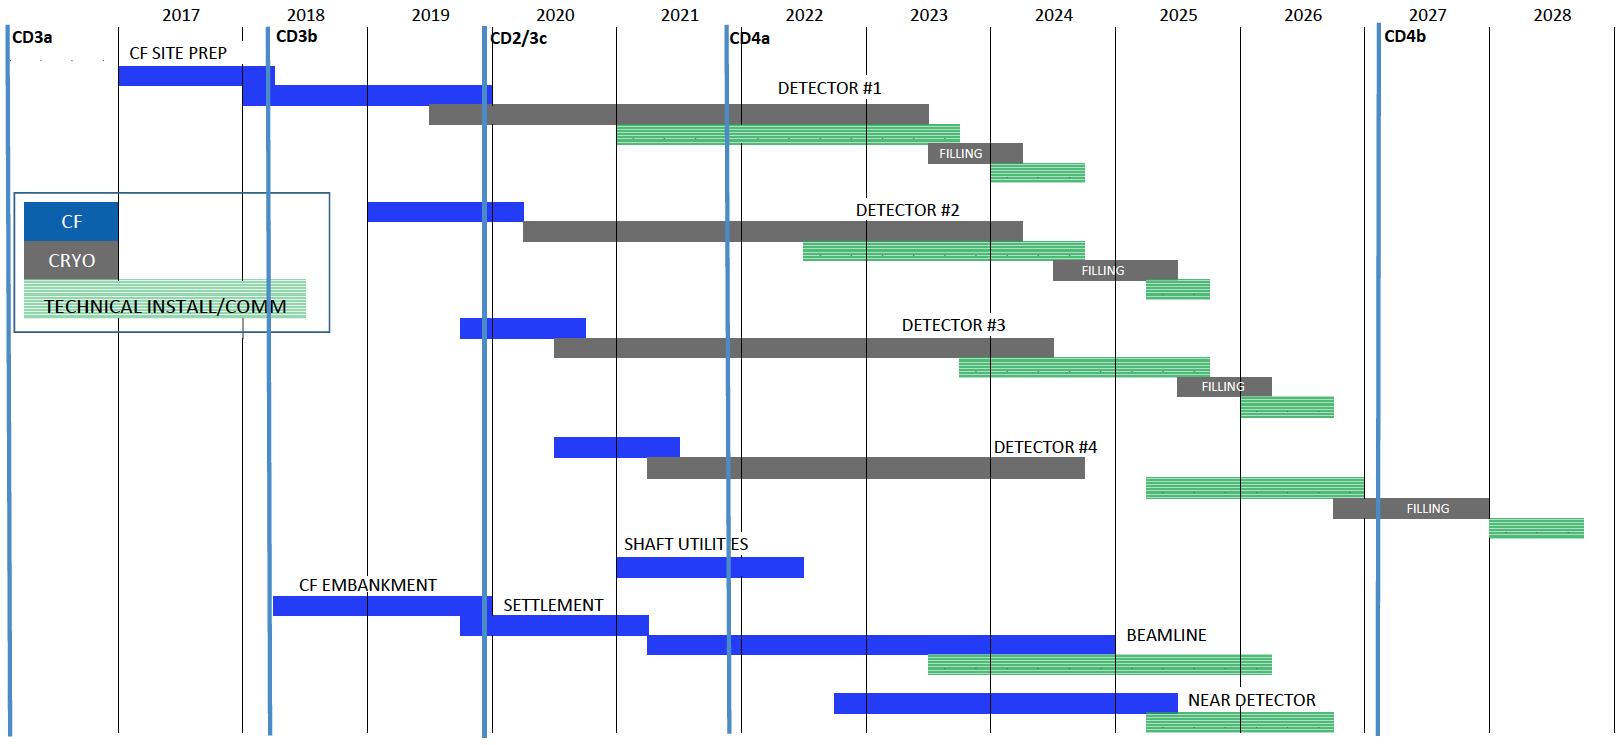
\includegraphics[width=1.2\textwidth, angle=90]{summary-schedule.png}
\end{cdrfigure}


Within the anticipated DOE funding profile, in particular during the initial phase of the Project, the far site conventional
facilities are advanced first; their final design starts in early 2016. Early site preparation is timed to be completed 
in time to start excavation when the Ross Shaft rehabilitation work finishes
 in late 2018.   As each detector 
 cavern is excavated and sufficient utilities are installed, the cryostat and cryogenics system work proceeds, followed by detector installation, filling and commissioning. 
 The far detector module \#1 is to be operational by 2024  with modules \#2 and \#3 completed
 one and two years later, respectively, and module \#4 completed by early 2028.  

The near site work is delayed with respect to the far site due to the anticipated funding profile. The near site CF and beamline work essentially slows to nearly a stop 
until design restarts in late 2017. Optimization decisions about the beamline that affect the CF design will need to be made by late 2018 in order to be ready for the CF design process. The embankment is constructed and then allowed to settle for at least twelve months before the majority of the beamline CF work proceeds. The beneficial occupancies of the various beamline facilities  
are staggered to allow beamline installation to begin as soon as possible. With this timescale, the far detector science program  
starts with the first module installed and no beam, focusing on non-accelerator-based science  
for slightly more than one year until 
the beamline installation is completed.


The near detector CF construction overlaps that for the beamline, but lags due to available funding. The near detector assembly begins on the surface before beneficial occupancy, after which the detector is installed, complete at about the same time as far detector module \#4. 

The DOE project management process requires approvals at Critical Decision milestones, which allow the LBNF/DUNE Project to move to the next step. In fall 2015 the far site CF will seek approval for CD-3a Initial Far Site Construction to include some of the CF at SURF. In summer 2018 LBNF near site CF will seek CD-3b construction approval for Advanced Site Preparation to build the embankment. In 2019  LBNF and DUNE will seek to baseline the LBNF/DUNE scope of work, cost and schedule, as well as construction approval for the balance of the Project scope of work. 
The Project concludes with CD-4 approval to start operations.

